%\documentclass{article}
\documentclass[10pt]{article}
\usepackage{times}
%\usepackage{natbib}
%\usepackage{multicol}
\RequirePackage{natbib}
\usepackage{amsmath, amssymb, fullpage, amsthm, array,,graphicx,asa, url}
%\usepackage[dvips]{graphics}

%\usepackage{hyperref} % for hyper reference

\graphicspath{{images/}}

% \usepackage{pifont} % this package is used to print check mark \checkmark
% \linespread{1.6} % factor 1.6 = double space

%\usepackage{setspace}
%\doublespacing



\setlength{\oddsidemargin}{0in}
\setlength{\evensidemargin}{0in}
\setlength{\textwidth}{6.5in}
\setlength{\topmargin}{-0.4in}
\setlength{\textheight}{9in}
\evensidemargin 
\oddsidemargin

\newtheorem{thm}{Theorem}[section]
\newtheorem{dfn}{Definition}[section]
\newtheorem{cor}{Corollary}[thm]
\newtheorem{con}{Conjecture}[thm]
\newtheorem{lemma}[thm]{Lemma}

%\topmargin -0.10in   % when making pdf
%\textheight 9.15in  % when making pdf

\pdfminorversion=4 % as instructed by JASA file upload


\begin{document}

\tableofcontents

% Article top matter
\title{Impact of Demographics and Skills of the Observer on Visual Statistical Inference }
\author{{Mahbubul Majumder, Heike Hofmann, Dianne Cook}
\thanks{Mahbubul Majumder is a PhD student (e-mail: mahbub72@gmail.com) , Heike Hofmann is an Associate  Professor and Dianne Cook is a Professor in the Department of Statistics and Statistical Laboratory, Iowa State University, Ames, IA 50011-1210. This research is supported in part by the National Science Foundation Grant \# DMS 1007697.}}
\date{\vspace{-.5in}}
%\date{\today}  %\today is replaced with the current date
\maketitle

\begin {abstract}  
Visual Inference is dependent on the careful evaluation of the lineups by individual observers. Each individual is different in their cognitive phycology and judiciousness which can affect the power of visual inference. To estimate the power of visual inference this can be controlled by getting evaluations from multiple people from a diverse population. But the other factor that may affect the power of visual inference is the demographics and skills of the observer. In this paper we examine this in details. The simulation experiments suggest that individual skill as well as demographics are very significant for the power of visual inference. Moreover, the data shows the evidence of learning or getting skilled while sequentially evaluating multiple lineups.

{\bf Keywords: \sf statistical graphics, lineup, non-parametric test, cognitive phycology, visualization, exploratory data analysis} 
\end {abstract}

%\begin{multicols}{2}
%\twocolumn

\section{Introduction} 

The fundamental concept of visual statistical inference is introduced by \citet{buja:2009} and later these concepts are validated by \citet{majumder:2012}.

\subsection{Visual Inference} A short introduction of visual inferential procedure.
\subsection{Estimation of Power of Visual Inference} Discussion of the methods for estimating the power of visual inference \citep{majumder:2012}. 

\section{Factors Affecting the Power of Visual Inference} A brief description of the factors that may affect the power of visual inference.

\subsection{Choice of Visual Test Statistic} Visual test statistics as defined in \citep{majumder:2012} serve two main purposes. One is to display a prominent pattern that should direct the human observers to select the actual plot in the lineup when the null hypothesis is not true. The another feature is that it should not show any strange pattern when null hypothesis is true, i.e., it should show similar pattern that null plots may have. Thus a visual test statistic is highly associated with the hypothesis. To achieve these purposes it is very important to decide which plot type and plot features should be adopted. As discussed in \citep{majumder:2012} following grammar of graphics developed  by \citet{wilkinson:1999} and later improved by \citet{hadley:2009} can give the task a standard control. 

Some of the effective features of visual test statistics are discussed in \citep{heike:2012} including plot type, color and shape of the plots. It is also observed that a scatterplot may do a better job than a box plot when using as a visual test statistic for regression parameters \citep{majumder:2012} .  \citep{niladri:2012} presents some \textit{distance measure} to determine how a plot may be different from another.

Plots to do: for the same signal strength show the proportion correct for scatterplot and boxplot. eg., qplot(effect, ump-visual power, color= plot-type)

\subsection{Question that Human Observer Answers} When a observer is prepared to evaluate a lineup, there needs to be a guideline what exactly should be looked for in a lineup. The researcher knows about the hypothesis but the observer does not know the underlying details of the lineup. Thus the researcher needs to ask a question observer needs to answer while evaluating the lineup. This question should provide the observer a little clue so that the answer reflects the hypothesized patterns in the actual plot. For example Table \ref{tbl:visual_stat} shows the questions asked for the simulation experiments done by  \citet{majumder:2012}. Notice that for case 1 if the observer can identify the actual plot in the lineup that should indicate that the plot chosen has the most vertical difference between groups A and B which is exactly what the researchers intend to examine. Similarly for case 2, a correct evaluation would indicate that the slope is different than the slope that may show up just from randomness.


\begin{table*}[hbtp] 
\caption{Visual test statistics and question asked to the observers to answer while evaluating a lineup } 
\centering 
\begin{tabular}{m{0.5cm}m{2cm}m{3cm}m{7.5cm}} 
\hline\hline 
Case & Statistic & Test Statistic & Lineup question \\ [0.5ex] % inserts table %heading 
\hline 
1  & Box plot & \begin{minipage}[t]{3cm} 	\scalebox{0.45}{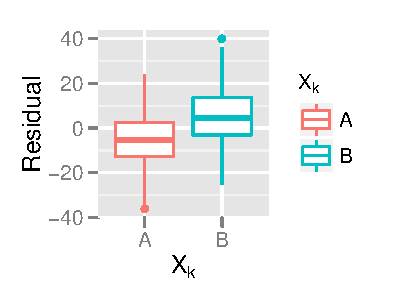
\includegraphics{stat_category.pdf}} \end{minipage} & Which set of box plots shows biggest vertical difference 
between group A and B? \\
2 &  Scatter plot & \begin{minipage}[t]{3cm}   \scalebox{0.45}{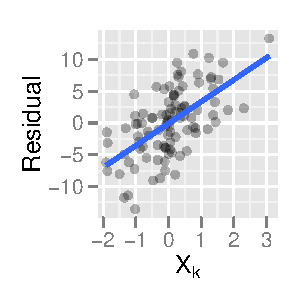
\includegraphics{stat_beta_k.pdf}}\end{minipage} & Of the scatter plots below which one shows data that has steepest slope? \\ 

\hline 
\end{tabular} 
\label{tbl:visual_stat} 
\end{table*} 

These questions are very crucial for the power of visual test. They help observer think in a controlled direction. Notice that there may be unnecessary patterns in the actual data plot which may not necessarily indicate the existence of the significant signal in the plot. These question help observer not to be misguided by those patterns. To review further on this \citet{majumder:2012} have also asked why the observers choose a specific plot. 



\subsection{Observer Personality} Each person is different from others in some way. For example, in a controlled experimental study \citet{zhao:2012}  notice that some people spend a lot of time to decide no matter whether the lineup is difficult or easy while some simply glance at lineups to make a decision. This influences the response of the observer and we see the subject specific variation in the power of visual test \citep{majumder:2012}. 

\subsection{Visual Perception of Human Eye} Different people observe the lineup in different ways.  With the help of eye-tracking equipment \citet{zhao:2012} track the observers' eyes to see how they go through the plots in a lineup to come to their answers. The result suggest that people have particular methods of reading lineups. Some people read lineups from left to write direction while some read from upward to downward. Some people start looking from the center of the lineup while others start from the top left corner. In the earlier phase of the exercise, the observer tend to scan the plots and then start comparing plots to make a final decision. Beside right-left or up-down directions observer show some diagonal movement too. 

Given this pattern of human eye tracks, it may effect the performance of an observer depending on where the actual plot is placed in the lineup. If the actual plot is on the top left corner and the observer starts from that point it may be easier to detect the actual plot earlier in the exercise and the observer could get plenty of time to make comparison. Thus the position of the actual plot in a lineup has some impact.


\subsection{Demographics of Observer}  Age, gender and location of the observer.
\subsection{Skills of Observer} Knowledge about statistical plot as well as education level.

\section{Simulation Experiment for Learning Effect}

\subsection{Experiment Setup} Description of the simulation experiment giving focus on demographics and skills of experimental subjects.
\subsection{Estimation of sample size}  How the sample size is estimated
\subsection{Data collection methods}  Description of the simulation experiment giving focus on demographics and skills of experimental subjects.
\subsection{Amazon Mechanical Turk}

Amazon Mechanical Turk \cite{turk} is an online work place where people from around the world can perform simple task to get paid. Usually tasks are very simple and no specialized training is required. Being a human is the main requirement. The tasks are designed such that it does not take much time to complete. Humans are still better than computers in performing these types of tasks. The the amount of money paid for each task is very small as well. Figure \ref{fig:amazon_task} displays an example of such a task.

\begin{figure}[htbp] 
   \centering
   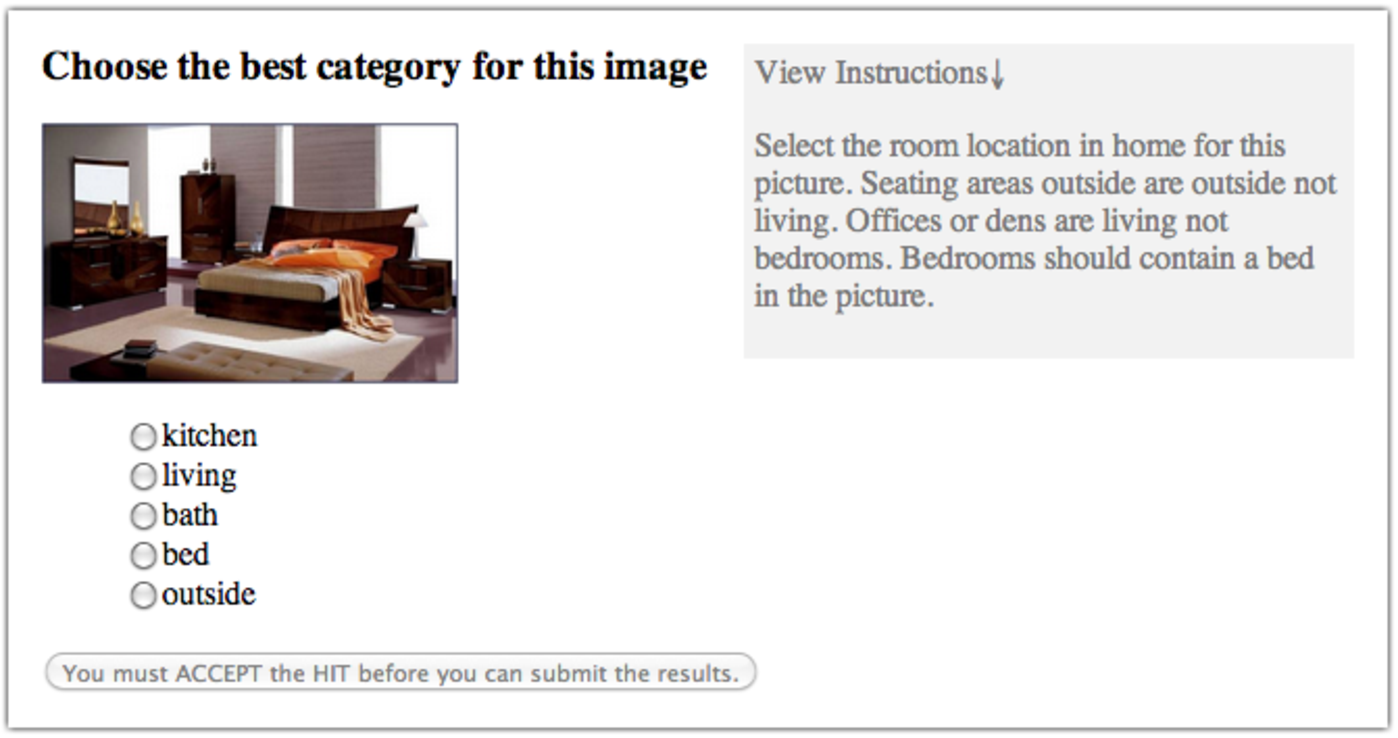
\includegraphics[width=5in]{amazon_task.pdf} 
   \caption{An example of amazon mechanical turk task. Tasks are usually very simple and human are still better than computer in performing these types of tasks. With each task, simple instructions are given for workers to follow. The workers first accept the task before submitting their response.}
   \label{fig:amazon_task}
\end{figure}

\section{Results}
\subsection{Overview of the Data}
\subsection{Diversity of the Experimental Subjects} Amazon Mechanical Turk \cite{turk} web site is a good source for recruiting people to evaluation lineups. It is a source of diverse workers who can give us feedback on visual inspection. This is the kind of task where human are better than computers.  Figure \ref{fig:turker_location} shows the location from where we received data. Notice that we received data from around the world and we observed diversity of location in the collected data. We notice diversity in not only location of the observers but also their gender, age groups and education levels. Table \ref{} shows that we have data from almost similar size of male and female population. 

\begin{figure}[htbp] 
   \centering
   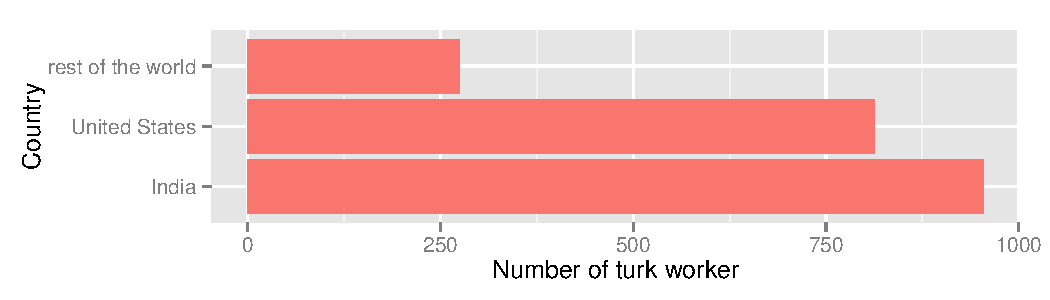
\includegraphics[width=4in]{turker_country.pdf} 
   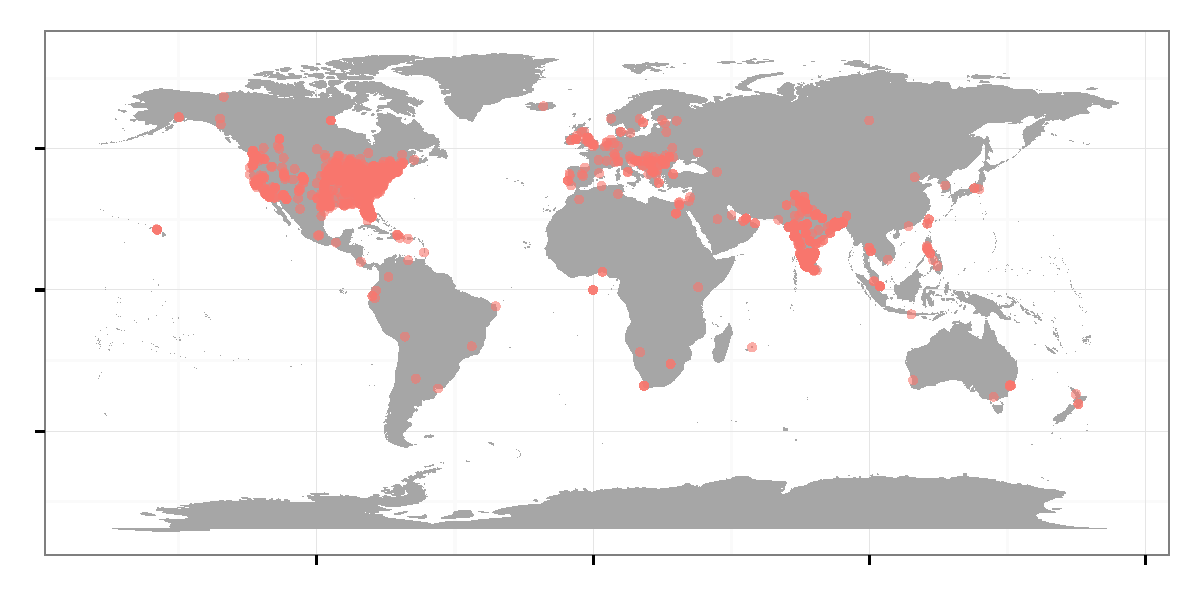
\includegraphics[width=4in]{turker_location.pdf}    
   \caption{Words used to explain the reasons for selection of data plot in a lineup. Larger font indicate more people choosing that word. Different color is used just to separate the words.}
   \label{fig:turker_location}
\end{figure}

\subsection{How people pick the data plot} In the experiment setup we have a question for the turk observers to choose the reason for their selection of a particular data plot. It is shown by \cite{majumder:2012} that these choice reasons reveal the way people picks the data plot in the lineup. To investigate this further we added free text input option for their choice reason instead of some fixed reasons to select from. In this experiment people could write whatever they think their reasons for choice are. Figure \ref{fig:wordle} shows the words used to explain their reasons for choice. The most common words used to explain their choice are points and green which indicates two important feature of a plot. One is the indicator of plot aesthetics and the other is the color. Spread, steepest, line and apart are some other important words used frequently. Spread and apart are indicative of variability in the data. Steepest and line indicates some sort of systematic pattern in the data.

\begin{figure}[htbp] 
   \centering
   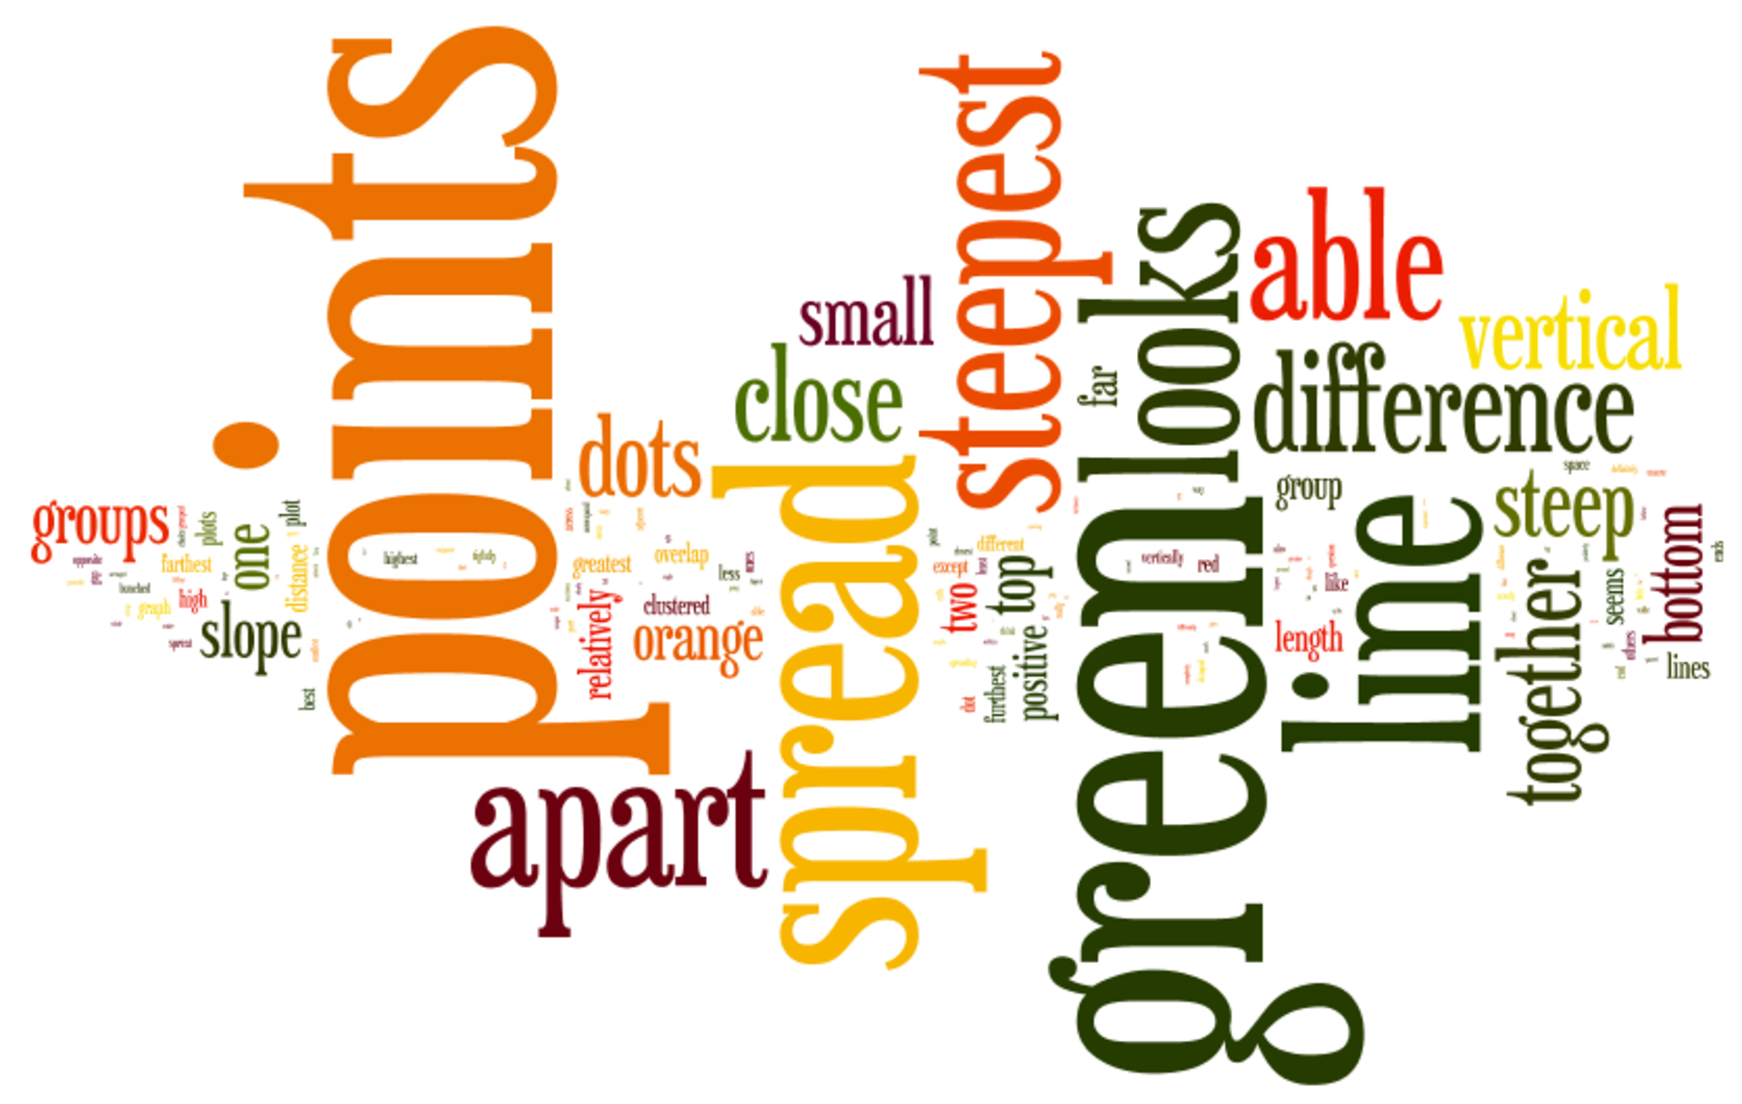
\includegraphics[width=3.5in]{reasoning_words.pdf} 
   \caption{Words used to explain the reasons for selection of data plot in a lineup. Larger font indicate more people choosing that word. Different color is used just to separate the words.}
   \label{fig:wordle}
\end{figure}

Figure \ref {fig:wordle} aslo shows some insight about peoples way of reading a plot. We notice that variability in the data, color and aesthetics used to generate plots and existence of any systematic pattern in the plot are some of the important features revealed from the figure. These features are commonly used by human brain to examine and compare plots. Notice that these features may be specific to this particular experiment. There could be different other features people would use to evaluate a lineup depending on the situation. But these words we have a general idea how people may think to evaluate a lineup.

\subsection{Learning Trend of the Observer} Since each subject is shown multiple lineups, they have a chance for self learning and do better on lineups shown later in the sequence. We examine this by fitting generalized mixed effect model presented in \cite{majumder:2012} with covariates attempt number and $p$-value of the lineup. The $p$-value of the lineup measures some sort of difficulty and including this should adjust for the difficulty level of the lineup while estimating the probability of correct responses in each attempt. Figure \ref{fig:learning_trend} shows the fitted subject wise learning pattern as well as overall learning pattern for each of the experiments. The parameter estimates of the model are shown in Table \ref{tbl:model_par}.

\begin{figure}[htbp] %  figure placement: here, top, bottom, or page
   \centering
   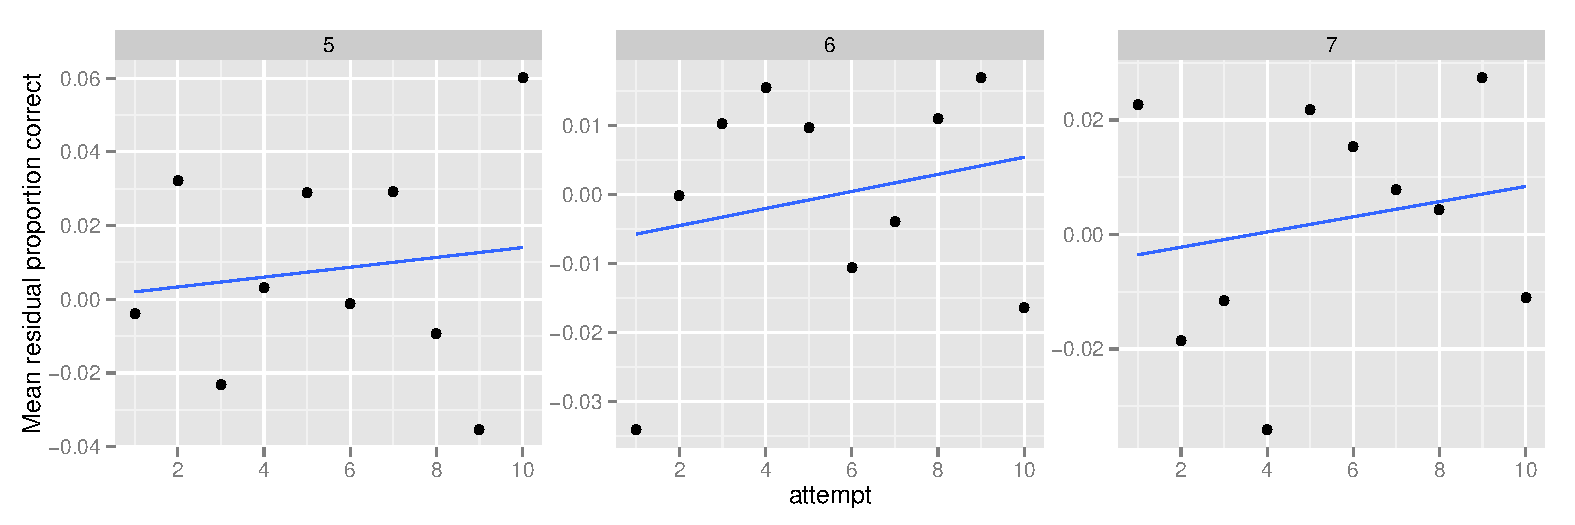
\includegraphics[width=4in]{learning_trend.pdf} 
   \caption{Mean absolute residuals vs attempt obtained by adjusting for lineup and subject specific variation. The trend over attempt does not show any learning trend since the slopes are not statistically significant.}
   \label{fig:learning_trend}
\end{figure}

\subsection{Location Effect of Data Plot in the Lineup}

We set up a Turk experiment to examine whether there is any difference of performance based on the location of actual data plot in the lineup. For this five locations of a lineup were randomly chosen to put the same actual data plot. The locations are 2,9,12,16,20 for Interaction effect and 1,8,12,17,20 for Genotype effect. For a lineup with specific data plot location, five sets of null plots are used giving 5 lineups for each location. In total we have 25 lineups for Interaction effect and 25 lineups for Genotype effect. These 50 lineups are then evaluated by 100 people recruited from Amazon Mechanical Turk. Each person evaluated 3 lineups one from Interaction, one from Genotype and the third one was a test lineup. The test lineup is used to process the payment and examine the quality of the data and the responses of the test plot is not added to our analysis. 

The proportion of correct responses by the turk observers are shown in Figure \ref{fig:location_effect}. Notice that the data plot is same for each location but we see some variability of performance based on different null plots. This may happen if some null plots appear to be more similar to the actual plot while the others are not making some lineups harder than others even though the actual data plot is same. This pattern is evident in the Figure \ref{fig:location_effect} as we see proportion correct for null plot 5 is consistently above the null plot 1 for each of the locations. But this variability could be controlled at some extent by collecting more data for each location. Since the variability is larger when we have small number of responses as we see in the figure. For example, we have only one response for null plot 3 and 5 for Interaction effect which should lead to the extreme proportion of correct since one response would either be correct or wrong. 

\begin{figure}[htbp] 
   \centering
    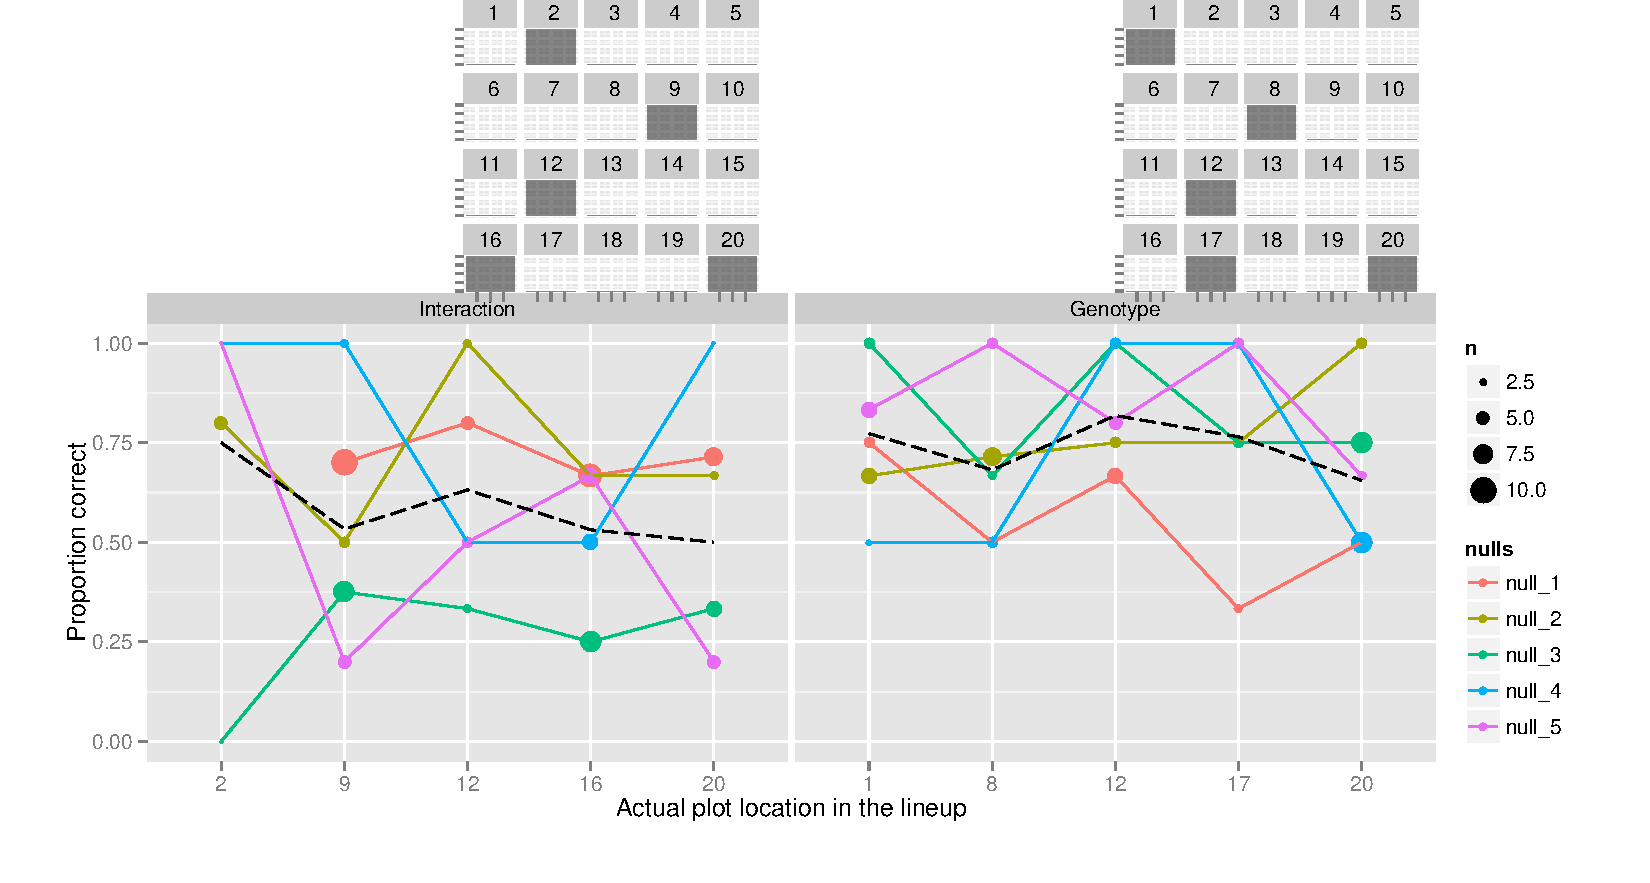
\includegraphics[width=6.5in]{proportion_nulls_guide.pdf} 
   \caption{Location of data plot in the lineup and proportion correct for both Interaction and Genotype effect. Each colored line represents a null set and the size of the dots represents number of responses. The overall average proportions are shown by dashed line. The actual data plot locations are shaded grey on the top panels to demonstrate their relative positions on a lineup.}
   \label{fig:location_effect}
\end{figure}

It is also interesting to check whether the proportion correct differs if the actual plot is on the outer boundary of the lineup or inside the outer boundary. As we see in Figure \ref{fig:location_effect}, location 9, 12 are inside for Interaction effect and location 8, 12 are inside for Genotype. It does not appear to have any difference whether the actual plot is inside or outer border of the lineup.

The overall proportion of correct response does not seem to vary much for different location indicating the non-existence of location effect. Since the actual data plot is same for each of the null sets of plot, the response data constitutes a multivariate response. Thus, to examine if the difference in proportion correct among the locations is statistically significant we fit a one way multi variate analysis of variance (MANOVA) model to the data.

 Suppose $Y=(Y_1,Y_2, ... , Y_p)$ is a vector of random variable with dimension $p=5$ representing the response for five null sets. let $Y_{ij}$ represents $jth$ vector response for $ith$ location with $i=1,2, ..., 5$. We fit the following MANOVA model 
\begin{equation}\label{manova}
Y_{ij} = \mu_{i} + \epsilon_{ij}
\end{equation}
where $\mu_{i}= (\mu_{1i},\mu_{2i}, ..., \mu_{pi})$ is the mean vector for location $i$ and $Var(\epsilon_{ij})=\Sigma$. 

Model \eqref{manova} enables to test if the mean vectors are similar for different locations. To fit the model we use anova function of stats package of \cite{R:2012}. The results are shown in Table \ref{tbl:manova}. The $p$-values for both Interaction and Genotype effect are much bigger than the conventional threshold of 0.05 and we failed to reject the hypothesis that there is no difference in location. 

\begin{table}[hbtp]
\caption{The results obtained by fitting MANOVA Model \eqref{manova}.}
\begin{center}
\begin{tabular}{ccccccccc}
  \hline \hline
 Location & && & \multicolumn{3}{c} {Degrees of Freedom}  & F test \\
 \cline{5-7}
 Effect & DF & Pillai & Approx. F & Numerator& Denumerator &Residual & p value\\
  \hline
  Interaction& 3&1.4783 &0.7772&15&12 & 6 & 0.6821 \\ 
  Genotype &4&1.7796 &1.1221&20&28 & 8 &  0.3824 \\ 
   \hline
\end{tabular}
\end{center}
\label{tbl:manova}
\end{table}

We also fit Model \eqref{manova} with only two locations based on outer or inner plot location. By outer location we mean the data plot location which is on the border area of the lineup. For example inner locations of a lineup would be 7,8,9,12,13,14. It turns out that inner and outer locations are also not significantly different.

     



%\begin{table}[hbtp]
%\caption{Parameter estimates of mixed model. Estimates are highly significant with $p$-value $<$  0.0001 for all three experiment data.}
%\begin{center}
%\begin{tabular}{cr@{.}lcc}
%  \hline \hline
% &  \multicolumn{3}{c} {Fixed effect}  & Random effect\\
% \cline{2-4}
% Experiment & \multicolumn{2}{l}{Estimate}  &Std. error & Variance\\
%  \hline
%  1 & 0&39 & 0.0094 & 0.0080 \\ 
%  2 & 1&21 &  0.0197 &  0.0443 \\ 
%  3 & 0&59 (Intercept)  &   0.1668 & 1.9917\\ 
%     & 0&21 (Slope)    &  0.0511     &  0.0245\\ 
%     &-0&78 (correlation) & & \\
%   \hline
%\end{tabular}
%\end{center}
%\label{tbl:model_par}
%\end{table}




% latex table generated in R 2.15.0 by xtable 1.7-0 package
% Fri Sep  7 10:28:47 2012
\begin{table}[hbtp]
\caption{Fixed effect parameter estimates of generalized mixed model. Note that attempt is not significant for experiment 2. The continuous covariate, lineup difficulty, was measured by the $p$-value of the actual plot in the lineup.}
\begin{center}
\begin{tabular}{llrrrrl}
  \hline
& Parameters & Estimate & Std..Error & z.value & P-value  & \\ 
  \hline
\multicolumn{2}{l}{\bf{Experiment 1} } &&&& &\\
&(Intercept) & -0.30 & 0.10 & -2.89 & 0.00 & ***\\ 
 & attempt & 0.08 & 0.02 & 4.21 & 0.00 & ***\\ 
 & lineup difficulty & -11.32 & 1.01 & -11.19 & 0.00 & ***\\ 
\multicolumn{2}{l}{\bf{Experiment 2} } &&&&& \\
 & (Intercept) & 2.36 & 0.15 & 16.09 & 0.00 & ***\\ 
 & attempt & 0.01 & 0.03 & 0.35 & 0.72 \\ 
 & lineup difficulty & -55.03 & 2.20 & -25.00 & 0.00 & ***\\ 
\multicolumn{2}{l}{\bf{Experiment 3} } &&&& \\
 & (Intercept) & 0.25 & 0.16 & 1.58 & 0.11 & .\\ 
 & attempt & 0.10 & 0.03 & 3.34 & 0.00 & ***\\ 
 & lineup difficulty & 3.00 & 0.56 & 5.36 & 0.00 & ***\\ 
   \hline
\end{tabular}
\end{center}
\label{tbl:model_par}
\end{table}

% \footnote{Signif. codes: 0 �***� 0.001 �**� 0.01 �*� 0.05 �.� 0.1}




%\begin{figure}[htbp] %  figure placement: here, top, bottom, or page
%   \centering
%   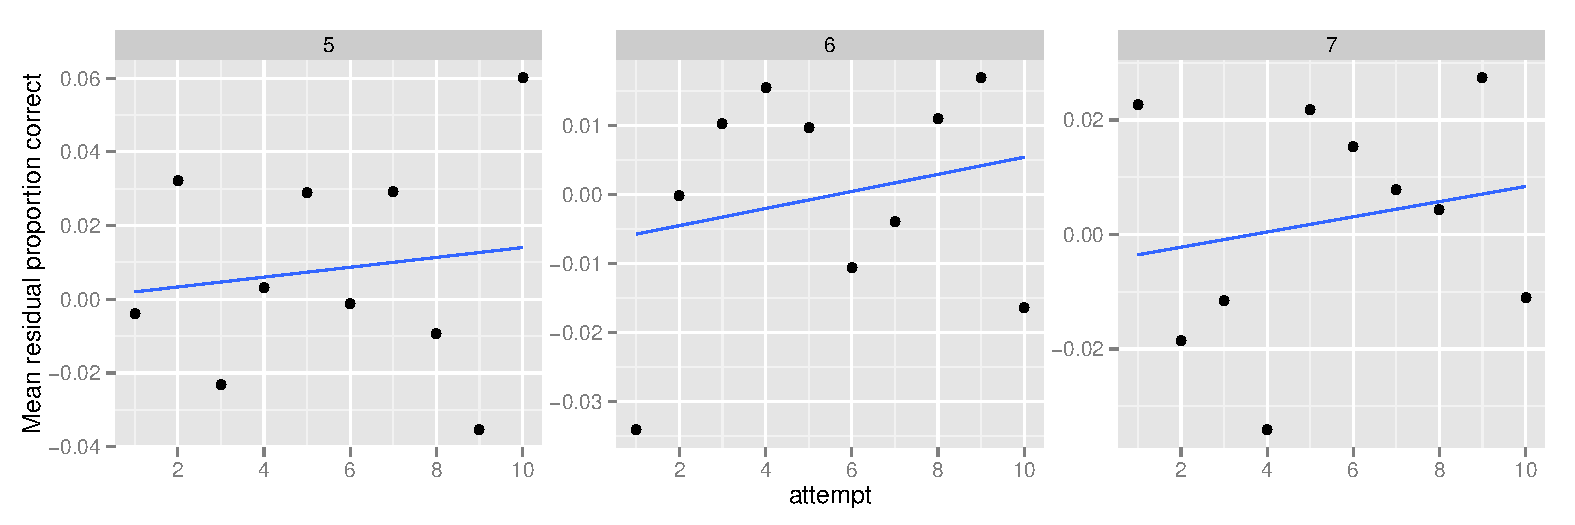
\includegraphics[width=4in]{learning_trend.pdf} 
%   \caption{Probability of correct response for different attempts by each subjects for a plot with lineup difficulty ($p$-value of actual plot) = 0.05 . The overall probability increases with attempts indicating a learning trend of the observers for experiments 1 and 3. For experiment 2 the overall trend is not statistically significant. Subject to subject variability is seen in learning pattern.}
%   \label{fig:learning_trend}
%\end{figure}

\section{Conclusion}


\bibliographystyle{asa}
\bibliography{references}

\end{document}



